\section{Реализация системы}

Реализация выполнена как набор сервисов на Java~25 и Spring Boot. Код размещён в Gradle monorepo: прикладные сервисы, protobuf-контракты и вспомогательные библиотеки собираются независимо, но используют единый набор соглашений по конфигурации, наблюдаемости и интеграции.

Взаимодействие синхронных контуров построено на gRPC. Асинхронная обработка команд доставки, статусов и fallback-событий выполняется через Kafka. Для транзакционных данных используются PostgreSQL-хранилища, для шаблонов --- MongoDB, для истории статусов --- ClickHouse. Redis используется только для TTL-механизмов: отметок отмены и локального подавления дублей в sender-сервисах.

\subsection{Обзор владения данными}

Хранилища разделены по сервисным границам. Сервис не читает таблицы или коллекции другого сервиса напрямую: доступ к данным выполняется через gRPC-контракт или через события Kafka. Такое разделение снижает связность схем данных и не превращает базу данных в общий интеграционный слой.

\begin{table}[h]
    \centering
    \footnotesize
    \renewcommand{\arraystretch}{1.15}
    \caption{Владение данными по сервисным контурам}
    \label{tab:data-ownership}
    \begin{tabular}{|L{0.22\textwidth}|L{0.18\textwidth}|L{0.36\textwidth}|L{0.16\textwidth}|}
        \hline
        \textbf{Сервис} & \textbf{Хранилище} & \textbf{Данные} & \textbf{Доступ других сервисов} \\
        \hline
        Notification Facade & Facade PostgreSQL & События уведомлений, аудитория, входные dispatch-запросы, outbox-записи и ключи идемпотентности. & Только через gRPC/Kafka \\
        \hline
        Template Registry & MongoDB Templates & Шаблоны, версии шаблонов, channel contents и activeVersion. & Через gRPC \\
        \hline
        Profile Consent & Profile Consent PostgreSQL & Профиль получателя, tenant-aware разрешения каналов, destination и ограничения. & Через gRPC \\
        \hline
        Delivery Dispatcher & Dispatcher PostgreSQL & Отложенные задачи, routing decisions, retry/fallback state и состояние планирования. & Через Kafka/gRPC \\
        \hline
        Cancellation Service & Redis Cancellation Marks & Отметки отмены dispatch/delivery с TTL 30 минут. & Через gRPC \\
        \hline
        Notification Mail Sender & Redis Mail Dedup & TTL-ключи локального dedup для email-команд. & Не используется другими сервисами \\
        \hline
        Notification SMS Sender & Redis SMS Dedup & TTL-ключи локального dedup для SMS-команд. & Не используется другими сервисами \\
        \hline
        History Writer & ClickHouse History Store & Append-only история статусов доставки и атрибуты обработки. & Через API history-writer \\
        \hline
    \end{tabular}
\end{table}

DBML-версии реляционных схем подготовлены отдельно в каталоге docs/dbdiagram. Они используются как источник для ERD-изображений в данном разделе; PlantUML-версии схем сохранены в каталоге docs/plantuml.

\subsection{notification-facade}

Notification Facade принимает клиентские команды, проверяет входные данные, фиксирует событие уведомления и аудиторию, подготавливает dispatch request и публикует его в Kafka topic delivery.dispatcher. В этом сервисе остаются операции, связанные с входным жизненным циклом события: идемпотентность клиентской команды, запись события, работа с аудиторией и формирование outbox-записей для последующей публикации.

Фасад не отправляет команды напрямую в mail- или sms-sender. После подготовки события он публикует общий dispatch request, а выбор канала и fallback-решения выполняет delivery-dispatcher. При клиентской отмене фасад вызывает cancellation-service и не хранит отметки отмены в собственной PostgreSQL-схеме.

Основные таблицы фасада отражают входное событие, адресатов, dispatch-запрос и outbox. Реляционная модель приведена на рисунке~\ref{fig:data-facade-postgres-schema}.

\begin{figure}[H]
    \centering
    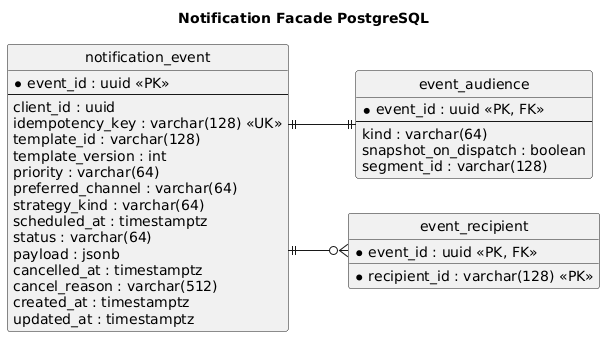
\includegraphics[width=0.82\textwidth]{inc/dbdiagram/png/facade-postgres-schema.png}
    \caption{Реляционная модель notification-facade}
    \label{fig:data-facade-postgres-schema}
\end{figure}

\subsection{template-registry}

Template Registry отвечает за хранение и рендеринг шаблонов уведомлений. Сервис получает от фасада идентификатор шаблона, канал и параметры рендеринга, выбирает активную версию и возвращает подготовленное содержимое. Модель хранится в MongoDB, потому что документ шаблона содержит версии, канальные представления и набор переменных, которые удобнее хранить как вложенную структуру.

В документе шаблона фиксируются client id, template id, activeVersion и набор версий. Для каждой версии хранятся channel contents для email и SMS, тема, тело и metadata. Пример структуры документа показан на рисунке~\ref{fig:data-template-registry-mongo}.

\begin{figure}[H]
    \centering
    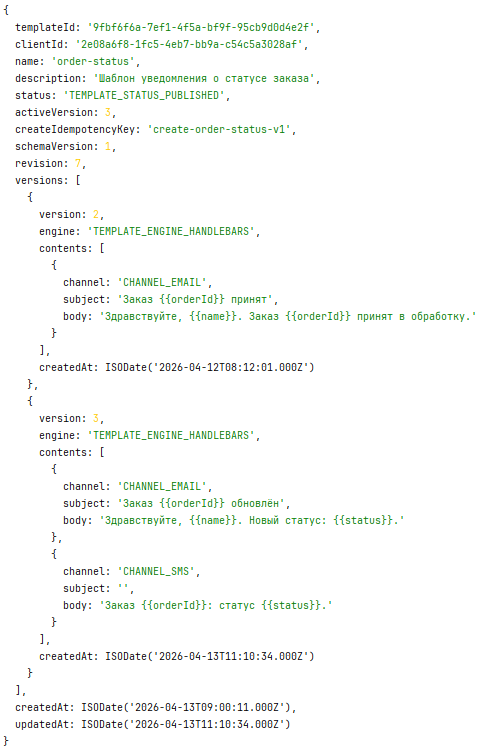
\includegraphics[width=0.76\textwidth]{inc/mongo-template-data.png}
    \caption{Модель MongoDB-документа template-registry}
    \label{fig:data-template-registry-mongo}
\end{figure}

\subsection{profile-consent}

Profile Consent инкапсулирует правила доступности каналов и профиль получателя. Delivery Dispatcher и другие сервисы не обращаются к таблицам профиля напрямую: они используют gRPC-метод проверки канала. Это сохраняет единое место принятия решений по recipient/channel/tenant.

PostgreSQL используется как транзакционное хранилище долговременных настроек профиля, согласий, channel destination и признаков блокировки. Основная таблица фиксирует активность профиля и предпочтительный канал, а таблица согласий хранит пару channel-tenant, destination, признак enabled и блокировку. Реляционная модель profile-consent приведена на рисунке~\ref{fig:data-profile-consent-postgres-schema}.

\begin{figure}[H]
    \centering
    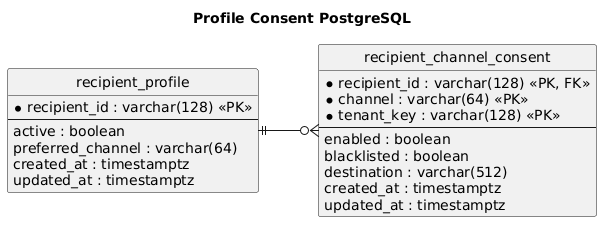
\includegraphics[width=0.82\textwidth]{inc/dbdiagram/png/profile-consent-postgres-schema.png}
    \caption{Реляционная модель profile-consent}
    \label{fig:data-profile-consent-postgres-schema}
\end{figure}

\subsection{delivery-dispatcher}

Delivery Dispatcher потребляет dispatch requests из delivery.dispatcher и fallback events из delivery.fallback. Сервис управляет отложенным запуском, принимает routing-решение, проверяет профиль и согласия через profile-consent, публикует команды в канальные Kafka topics и защищает fallback от бесконечного цикла.

Dispatcher не выполняет входную бизнес-валидацию, не работает с аудиторией и не рендерит шаблоны. Эти операции остаются в notification-facade. Его зона ответственности начинается после появления валидного dispatch request в Kafka и ограничена оркестрацией доставки, планированием и маршрутизацией.

Собственная PostgreSQL-модель dispatcher хранит планировочное состояние, routing decisions, retry/fallback state и технические данные, которые нужны для безопасного повторного запуска. Схема показана на рисунке~\ref{fig:data-dispatcher-postgres-schema}.

\begin{figure}[H]
    \centering
    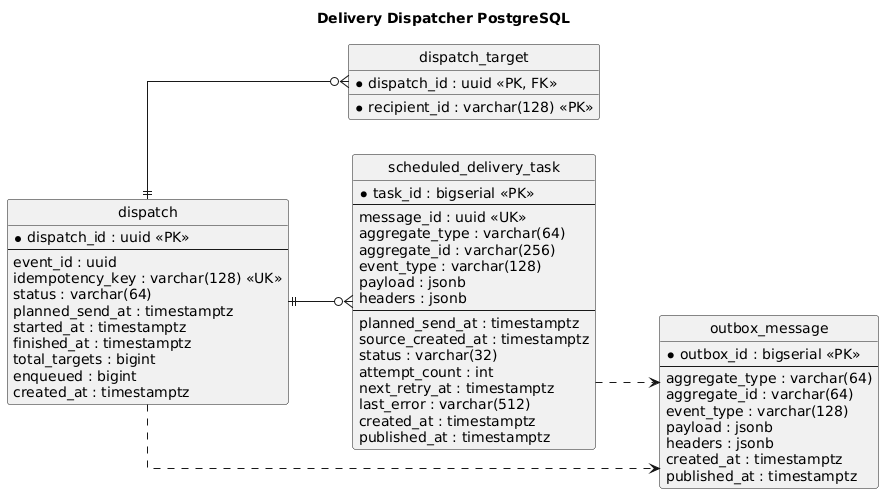
\includegraphics[width=0.86\textwidth]{inc/dbdiagram/png/dispatcher-postgres-schema.png}
    \caption{Реляционная модель delivery-dispatcher}
    \label{fig:data-dispatcher-postgres-schema}
\end{figure}

\subsection{cancellation-service}

Cancellation Service выделен в отдельный контур, потому что отмена dispatch/delivery должна быстро проверяться sender-сервисами перед обращением к внешнему провайдеру. Сервис предоставляет gRPC-методы фиксации отмены и проверки допустимости отправки.

Отметка отмены хранится в Redis как TTL-key. Время жизни ключа составляет 30 минут: после этого окно практической отмены считается закрытым, а дальнейшая судьба доставки определяется обычным статусным контуром. Повторный запрос отмены обрабатывается идемпотентно. Если sender получает признак отмены, он не вызывает внешний provider API и публикует статус CANCELED.

\subsection{notification-mail-sender}

Notification Mail Sender потребляет email-команды из Kafka и выполняет только execution-level проверки. Перед отправкой сервис атомарно записывает Redis dedup key через операцию типа SET NX EX, затем обращается к cancellation-service. Если доставка отменена, внешний email provider не вызывается, а в Kafka публикуется статус CANCELED.

Если отмены нет, sender выполняет отправку через SMTP/provider API и публикует итоговый статус. При окончательной ошибке email-канала сервис не выбирает альтернативный канал самостоятельно. Он публикует fallback event в delivery.fallback, после чего решение принимает delivery-dispatcher.

\subsection{notification-sms-sender}

Notification SMS Sender устроен аналогично mail sender. Он потребляет SMS-команды, выполняет локальный Redis-based dedup, проверяет cancellation-service и только после этого вызывает SMS provider API. При отмене публикуется статус CANCELED; при технической ошибке фиксируется статус доставки через общий Kafka status pipeline.

SMS sender не владеет шаблонами, профилем получателя или правилами fallback. Эти решения остаются в template-registry, profile-consent и delivery-dispatcher соответственно.

\subsection{history-writer}

History Writer вынесен из online-path доставки и работает как потребитель status events из Kafka. Сервис записывает события статусов в ClickHouse в append-only модель. Такая схема позволяет отделить аналитическое чтение истории от транзакционных контуров notification-facade и delivery-dispatcher.

ClickHouse-таблица содержит идентификаторы события, dispatch и delivery, канал, статус, причину ошибки, номер попытки, время возникновения статуса и технические атрибуты Kafka-публикации. Модель хранения истории приведена на рисунке~\ref{fig:data-history-clickhouse-schema}.

\begin{figure}[H]
    \centering
    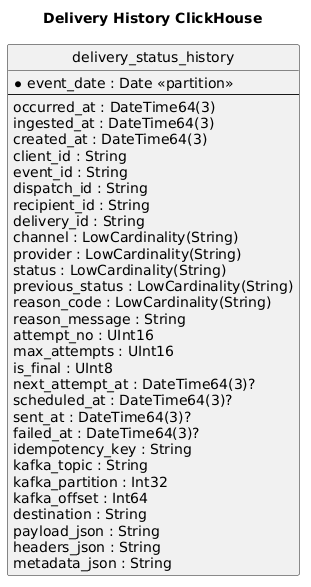
\includegraphics[width=0.38\textwidth]{inc/dbdiagram/png/history-clickhouse-schema.png}
    \caption{Модель хранения истории доставки в ClickHouse}
    \label{fig:data-history-clickhouse-schema}
\end{figure}
